
\section{\trAffineScheme{}的\trStructureSheaf}

现在我们想在\emph{任意}的\trOpenSet{}上给出一个由函数组成的环；但我们知道，只需把\trTopology{}的某组\trBase{}上的函数描述清楚便已足够。我们将会看到，由诸\trDistinguishedOpen{}组成的这组\trBase——下称\textbf{\trDistinguishedBase{}}（distinguished base）——会让事情比你可能惧怕的容易驾驭得多。于是我们现在就把\trStructureSheaf{}当作「诸\trDistinguishedOpen{}这组\trBase{}上的一个（环的）\trSheaf」来描述（\cref{thm:sheaves-recovered-from-base}与\cref{ex:distinguished-opens-base}）。

\begin{definition}\label{thm:structure-sheaf-definition}
我们把 $\OO_{\Spec A}(D(f))$ 定义为 $A$ 在如下\trMultiplicativeSubset{}上的\trLocalization：在 $V(f)$ 之外不消失的函数全体（即那些使 $V(g)\subset V(f)$、等价地使 $D(f)\subset D(g)$ 的 $g\in A$；对照\cref{ex:distinguished-open-inclusion}）。这一定义只依赖于 $D(f)$，而不依赖于 $f$ 本身。（研究空集的学者或许会注意到：由\cref{ex:distinguished-open-empty}可知 $\OO_{\Spec A}(\varnothing)=\{0\}$。）
\end{definition}

\begin{exercise}[极好练习]\label{ex:af-structure-sheaf-isomorphism}
证明自然映射 $A_f\to\OO_{\Spec A}(D(f))$ 是\trIsomorphism。（可能的提示：\cref{ex:distinguished-open-inclusion}。）
\end{exercise}

若 $D(f')\subset D(f)$，则按显而易见的方式定义\trRestrictionMap
\[
\mathrm{res}_{D(f),D(f')}\colon\OO_{\Spec A}(D(f))\longrightarrow\OO_{\Spec A}(D(f'))
\]
（后一个环正是前一个环的进一步\trLocalization）。诸\trRestrictionMap{}显然可以复合：这便是一个\trDistinguishedBase{}上的\trPresheaf。

\begin{theorem}\label{thm:sheaf-on-distinguished-base}
刚才描述的这份数据给出\trDistinguishedBase{}上的一个\trSheaf，从而在拓扑空间 $\Spec A$ 上确定出一个\trSheaf。
\end{theorem}

\textbf{4.1.3.}\quad 这个\trSheaf{}称为\textbf{\trStructureSheaf}，记作 $\OO_{\Spec A}$，当下标由上下文自明时也常简记为 $\OO$。此后，记号 $\Spec A$ 将指「一个\trTopologicalSpace{}连同其上的\trStructureSheaf」这份数据。这样的、连同\trStructureSheaf{}在一起的\trTopologicalSpace，称为\textbf{\trAffineScheme}（定义~4.3.1）。我们将继续沿用\trRingedSpace{}的语言（\S2.2.13）：\trOpenSet{}上的函数、\trGlobalSections，如此等等。\cref{thm:sheaf-on-distinguished-base}的重要教益不仅在于 $\OO_{\Spec A}$ 是一个\trSheaf，还在于\trDistinguishedBase{}为驾驭 $\OO_{\Spec A}$ 提供了一条上佳的途径。另请注意：我们由此为「把 $A$ 的元素解释为 $\Spec A$ 上的函数」给出了正当性。

\emph{证明。}\ 我们必须验证\trBase\trIdentityAxiom{}与\trBase\trGluability{}公理成立（\S2.5）。我们将对「整个空间 $\Spec A$」这个\trOpenSet{}验证二者，而把它们延伸到任意\trDistinguishedOpen{}的那个小窍门留给你（\cref{ex:base-identity-distinguished-open}与\cref{ex:base-gluability-distinguished-open}）。设 $\Spec A=\bigcup_{i\in I}D(f_i)$；等价地（\cref{ex:distinguished-cover-unit-ideal}），由诸 $f_i$ 生成的\trIdeal{}是整个环 $A$。

（旁注：熟悉 \S2.2.7 的\trEqualizer{}\trExactSequence{}的行家会意识到，我们正在证明的是下式的正合性：
\begin{equation*}\tag{4.1.3.1}\label{eq:equalizer-structure-sheaf}
0\longrightarrow A\longrightarrow\prod_{i\in I}A_{f_i}\longrightarrow\prod_{i\neq j\in I}A_{f_i f_j},
\end{equation*}
其中 $\{f_i\}_{i\in I}$ 是一族函数，满足 $(f_i)_{i\in I}=A$。右边的映射涉及正负号：映射 $A_{f_i}\to A_{f_i f_j}$ 是\trLocalization{}映射，而映射 $A_{f_j}\to A_{f_i f_j}$ 则是该\trLocalization{}映射的\emph{负}。\trBase{}恒等对应于在 $A$ 处的单性，\trGluability{}对应于在 $\prod_i A_{f_i}$ 处的正合性。）

我们先在\trBase{}上检验恒等性。设 $\Spec A=\bigcup_{i\in I}D(f_i)$，其中 $i$ 跑遍某个\trIndexSet{} $I$。那么存在 $I$ 的一个有限子集——我们把它命名为 $\{1,\dots,n\}$——使得 $\Spec A=\bigcup_{i=1}^{n}D(f_i)$，即 $(f_1,\dots,f_n)=A$（\cref{ex:distinguished-cover-finite-subcover}；这是 $\Spec A$ 之\trQuasicompactness{}的一个特例，见\cref{ex:spec-quasicompact}(a)）。设有 $s\in A$ 使得对一切 $i$ 都有 $\mathrm{res}_{\Spec A,D(f_i)}\,s=0$ 于 $A_{f_i}$ 中。我们要证 $s=0$。「$\mathrm{res}_{\Spec A,D(f_i)}\,s=0$ 于 $A_{f_i}$ 中」这一事实蕴涵：存在某个 $m$，使得对每个 $i\in\{1,\dots,n\}$ 都有 $f_i^{m}s=0$。现在 $(f_1^{m},\dots,f_n^{m})=A$（例如由 $\Spec A=\bigcup D(f_i)=\bigcup D(f_i^{m})$ 即得），于是存在诸 $r_i\in A$，使得 $\sum_{i=1}^{n}r_if_i^{m}=1$ 在 $A$ 中成立，从而
\[
s=\Bigl(\sum r_if_i^{m}\Bigr)s=\sum r_i(f_i^{m}s)=0.
\]
这样，我们就对 $\Spec A$ 验证了「\trBase{}恒等」公理。

\begin{exercise}\label{ex:base-identity-distinguished-open}
对上述论证稍作微调，证明\trBase{}恒等对任意\trDistinguishedOpen{} $D(f)$ 成立。（提示：在上述论证中恰到好处地把 $A$ 换成 $A_f$。）
\end{exercise}

接下来我们证明\trBase\trGluability。（塞尔曾把它描述为一种「\trPartitionOfUnity{}」\footnote{译注：\trPartitionOfUnity{}（partition of unity）是分析学中的标准工具：把常数 $1$ 表示成一族各管一方的非负函数之和。塞尔的比喻是说，下文构造 $r$ 时诸 $r_ih_i$ 恰好扮演了这些「份额」的角色。}式的论证；只要看的角度对，他的这个洞见极富启发。）再设 $\bigcup_{i\in I}D(f_i)=\Spec A$，其中 $I$ 是一个\trIndexSet{}（这个指标集可能无穷得可怕）。设在每个 $A_{f_i}$ 中各给定一个元素，它们在重叠 $A_{f_i f_j}$ 上相互一致。注意：诸\trDistinguishedOpen{}的交仍是\trDistinguishedOpen。

先设 $I$ 有限，比如说 $I=\{1,\dots,n\}$。我们有元素 $a_i/f_i^{\ell_i}\in A_{f_i}$，它们在重叠 $A_{f_i f_j}$ 上相互一致（见图~\ref{fig:base-gluability}(a)）。令 $g_i=f_i^{\ell_i}$；利用 $D(f_i)=D(g_i)$，把我们的元素视为形如 $a_i/g_i\in A_{g_i}$，便可简化记号（图~\ref{fig:base-gluability}(b)）。

\begin{figure}[htbp]
\centering
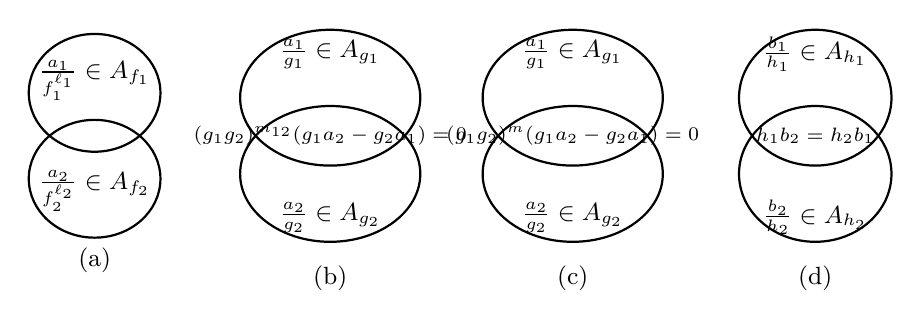
\begin{tikzpicture}[scale=0.88,every node/.style={font=\small}]
  \begin{scope}[shift={(0,0)}]
    \draw[thick] (0,0.62) ellipse (0.95 and 0.85);
    \draw[thick] (0,-0.62) ellipse (0.95 and 0.85);
    \node at (0,0.80) {$\frac{a_1}{f_1^{\ell_1}}\in A_{f_1}$};
    \node at (0,-0.80) {$\frac{a_2}{f_2^{\ell_2}}\in A_{f_2}$};
    \node at (0,-1.80) {(a)};
  \end{scope}
  \begin{scope}[shift={(3.4,0)}]
    \draw[thick] (0,0.55) ellipse (1.30 and 0.98);
    \draw[thick] (0,-0.55) ellipse (1.30 and 0.98);
    \node at (0,1.18) {$\frac{a_1}{g_1}\in A_{g_1}$};
    \node at (0,-1.18) {$\frac{a_2}{g_2}\in A_{g_2}$};
    \node at (0,0) {\scriptsize$(g_1g_2)^{m_{12}}(g_1a_2-g_2a_1)=0$};
    \node at (0,-2.05) {(b)};
  \end{scope}
  \begin{scope}[shift={(6.9,0)}]
    \draw[thick] (0,0.55) ellipse (1.30 and 0.98);
    \draw[thick] (0,-0.55) ellipse (1.30 and 0.98);
    \node at (0,1.18) {$\frac{a_1}{g_1}\in A_{g_1}$};
    \node at (0,-1.18) {$\frac{a_2}{g_2}\in A_{g_2}$};
    \node at (0,0) {\scriptsize$(g_1g_2)^{m}(g_1a_2-g_2a_1)=0$};
    \node at (0,-2.05) {(c)};
  \end{scope}
  \begin{scope}[shift={(10.4,0)}]
    \draw[thick] (0,0.55) ellipse (1.10 and 0.98);
    \draw[thick] (0,-0.55) ellipse (1.10 and 0.98);
    \node at (0,1.18) {$\frac{b_1}{h_1}\in A_{h_1}$};
    \node at (0,-1.18) {$\frac{b_2}{h_2}\in A_{h_2}$};
    \node at (0,0) {\scriptsize$h_1b_2=h_2b_1$};
    \node at (0,-2.05) {(d)};
  \end{scope}
\end{tikzpicture}
\caption{\trStructureSheaf{}的\trBase\trGluability{}。（依原书手绘图重绘。）}\label{fig:base-gluability}
\end{figure}

$a_i/g_i$ 与 $a_j/g_j$ 「在重叠上一致」（即在 $A_{g_i g_j}$ 中一致）意味着：对某个 $m_{ij}$，
\[
(g_ig_j)^{m_{ij}}(g_ja_i-g_ia_j)=0
\]
在 $A$ 中成立。取 $m=\max m_{ij}$（这里我们用到了 $I$ 的有限性），便可统一记号：
\[
(g_ig_j)^{m}(g_ja_i-g_ia_j)=0
\]
对一切 $i$, $j$ 成立（图~\ref{fig:base-gluability}(c)）。令 $b_i=a_ig_i^{m}$（对一切 $i$），并令 $h_i=g_i^{m+1}$（于是 $D(h_i)=D(g_i)$）。这样还能把记号简化得更彻底（图~\ref{fig:base-gluability}(d)）：在每个 $D(h_i)$ 上我们有函数 $b_i/h_i$，而重叠条件就是
\begin{equation*}\tag{4.1.3.2}\label{eq:overlap-condition-simplified}
h_jb_i=h_ib_j.
\end{equation*}
现在 $\bigcup_i D(h_i)=\Spec A$，由此知对某组 $r_i\in A$ 有 $1=\sum_{i=1}^{n}r_ih_i$。定义
\begin{equation*}\tag{4.1.3.3}\label{eq:r-gluing-definition}
r=\sum r_ib_i.
\end{equation*}
这个 $r$ 将就是那个限制到每个 $b_i/h_i$ 上的 $A$ 中元素。的确，由重叠条件 \eqref{eq:overlap-condition-simplified}，
\[
rh_j=\sum_i r_ib_ih_j=\sum_i r_ih_ib_j=b_j.
\]

接下来处理 $I$ 为无穷的情形：选取有限子集 $\{1,\dots,n\}\subset I$，使得 $(f_1,\dots,f_n)=A$（或者等价地，利用 $\Spec A$ 的\trQuasicompactness{}来选取 $D(f_i)$ 的一个有限子覆盖）。利用 \eqref{eq:r-gluing-definition}，如上构造 $r$。我们将证明：对任意 $z\in I-\{1,\dots,n\}$，$r$ 都限制到 $A_{f_z}$ 中我们想要的那个元素 $a_z/f_z^{\ell_z}$ 上。把上面的整个流程用 $\{1,\dots,n,z\}$ 代替 $\{1,\dots,n\}$ 再重演一遍，得到 $r'\in A$，它限制到 $a_i/f_i^{\ell_i}$（对 $i\in\{1,\dots,n,z\}$）。于是由\trBase\trIdentityAxiom，$r'=r$。（注意：我们是在用\trBase{}恒等来\emph{证明}\trBase\trGluability。这正是一个例证，说明恒等公理在某种意义上比可粘性公理更「在先」。）因此，$r$ 限制到 $A_{f_z}$ 中我们想要的那个元素 $a_z/f_z^{\ell_z}$ 上。

\begin{exercise}\label{ex:base-gluability-distinguished-open}
对上述论证作适当改动，证明\trBase\trGluability{}对任意\trDistinguishedOpen{} $D(f)$ 成立。
\end{exercise}

至此，\cref{thm:sheaf-on-distinguished-base}的证明便告完成。\hfill$\square$

\vkthmsync{4}
\begin{remark}[\hard\hard]\label{thm:sections-not-localization}
\cref{thm:structure-sheaf-definition}与\cref{thm:sheaf-on-distinguished-base}暗示了一种可能相当利落的办法，来描述 $\OO_{\Spec A}$ 在\emph{任意}\trOpenSubset{}上的\trSection：或许 $\OO_{\Spec A}(U)$ 就是 $A$ 在「在 $U$ 的任何一点处都不消失的函数全体」这个\trMultiplicativeSubset{}上的\trLocalization？这并不成立。一个反例（日后你将能使它精确化）：设 $\Spec A$ 为两份 $\mathbb{A}^2_k$ 沿其原点粘合所得的空间（显式方程见 (24.3.8.1)），并令 $U$ 为（诸）原点的补集。那么，在第一份 $\mathbb{A}^2_k\smallsetminus\{(0,0)\}$ 上取值 $1$、在第二份 $\mathbb{A}^2_k\smallsetminus\{(0,0)\}$ 上取值 $0$ 的那个函数，就不是这种形式。（追问：若粘合的是沿一点相贴的两份 $\mathbb{A}^1_k$，这套讨论为何就行不通了？）
\end{remark}

\textbf{4.1.5.\ 供日后使用的重要观念：由 $A$-模而来的 $\OO_{\Spec A}$-模。}\quad \cref{thm:sheaf-on-distinguished-base}的下面这个推广，对第~6~章中\trQCSheaf{}的定义将是必不可少的。你可以把这些练习留到那时再做，但趁这些想法在你脑海里还新鲜，现在就做也许最容易。

\begin{exercise}[重要练习兼定义]\label{ex:module-sheaf-on-base}
设 $M$ 是一个 $A$-\trModule。证明：下面的构造给出\trDistinguishedBase{}上的一个\trSheaf{} $\widetilde{M}$。定义 $\widetilde{M}(D(f))$ 为 $M$ 在「在 $V(f)$ 之外不消失的函数全体」这个\trMultiplicativeSubset{}上的\trLocalization；并照 $\OO_{\Spec A}$ 的情形完全类似地定义诸\trRestrictionMap{} $\mathrm{res}_{D(f),D(g)}$。证明这给出\trDistinguishedBase{}上的一个\trSheaf，从而给出 $\Spec A$ 上的一个\trSheaf。再证明这是一个 $\OO_{\Spec A}$-\trModule。
\end{exercise}

\vkthmsync{6}
\begin{remark}[重要注记]\label{thm:module-equalizer-exactness}
在解答上一练习的过程中，你将证明：若 $(f_i)_{i\in I}=A$，则
\begin{equation*}\tag{4.1.6.1}\label{eq:module-equalizer-sequence}
0\longrightarrow M\longrightarrow\prod_{i\in I}M_{f_i}\longrightarrow\prod_{i\neq j\in I}M_{f_i f_j}
\end{equation*}
（对照 \eqref{eq:equalizer-structure-sheaf}）是正合的。特别地，$M$ 可以等同于 $M_{f_1}\times\cdots\times M_{f_r}$ 的一个具体的\trSubmodule。尽管对每个 $f_i$ 而言 $M\to M_{f_i}$ 未必是\trInclusionMap，但 $M\to M_{f_1}\times\cdots\times M_{f_r}$ \emph{确实}是\trInclusionMap。这一点日后会派上用场：我们会想证明「若 $M$ 具有某条好性质，则 $M_f$ 也有」，那将很容易；我们还会想证明另一方向的推理：若 $(f_1,\dots,f_n)=A$ 且诸 $M_{f_i}$ 都有这条性质，则 $M$ 也有。这个想法将在\trAffineCommunicationLemma{}~5.3.2（Affine Communication Lemma）中得到精确表述。
\end{remark}

\begin{exercise}\label{ex:stalk-tilde-m-localization}
设 $\mathfrak{p}$ 是 $A$ 的一个\trPrimeIdeal。描述一个\trCanonical\trIsomorphism{} $\widetilde{M}_{[\mathfrak{p}]}\tilde{\longrightarrow}M_{\mathfrak{p}}$，它联系 $\widetilde{M}$ 的\trStalk{}与 $M$ 的\trLocalization。特别地，$\OO_{\Spec A}$ 在点 $[\mathfrak{p}]$ 处的\trStalk{}就是\trLocalRing{} $A_{\mathfrak{p}}$。
\end{exercise}

下面这条练习展示：一条重要的结论，从代数与几何两种视角去看，理解方式可以何等不同。

\begin{exercise}\label{ex:module-to-product-localizations}
设 $M$ 是一个 $A$-\trModule。证明自然映射
\[
M\lhook\joinrel\longrightarrow\prod_{\mathfrak{p}\in\Spec A}M_{\mathfrak{p}}
\]
是\trInjectiveMap，且有两种证法：(a)~考虑该映射的\trKernel，证明其中任何元素必为 $0$；(b)~把\cref{ex:sections-determined-by-germs}（\trSheaf{}的\trSection{}由\trGerm{}确定）应用到层 $\widetilde{M}$ 上。（于是：一个 $A$-\trModule{}是零，当且仅当它在所有\trPrimeIdeal{}处的\trLocalization{}都是零；而且我们看到，这同时是 (a)~一条代数事实与 (b)~一条几何事实。）
\end{exercise}

\begin{exercise}\label{ex:module-maps-sheaf-maps}
描述 $A$-\trModule{}之间的映射 $M\to N$ 与 $\OO_{\Spec A}$-\trModule{}之间的映射 $\widetilde{M}\to\widetilde{N}$ 之间的一个\trBijection。（换一种花哨的「翻译」：你这就把 $\catMod{A}$ 描述成了 $\catMod{\OO_{\Spec A}}$ 的一个\trFullSubcategory。）
\end{exercise}

\vkthmsync{7}
\begin{definition}[模的支撑]\label{thm:support-of-module}
受\cref{ex:stalk-tilde-m-localization}与「\trSheaf{}之\trSection{}的\trSupport{}」这一观念（\cref{thm:support-of-section}）的启发，定义 $\mathrm{m}\in M$ 的\textbf{\trSupport}为
\[
\Supp\mathrm{m}:=\{[\mathfrak{p}]\in\Spec A\ :\ \mathrm{m}_{\mathfrak{p}}\neq 0\}\subset\Spec A,
\]
即把 $\mathrm{m}$ 看作 $\widetilde{M}$ 的\trSection{}时的\trSupport。据\cref{ex:support-of-section-closed}，$\Supp\mathrm{m}$ 是 $\Spec A$ 的一个\trClosedSubset。
类似地（仿照\cref{thm:support-of-sheaf}），定义 $M$ 的\textbf{\trSupport}为
\[
\Supp M:=\Supp\widetilde{M}=\{[\mathfrak{p}]\in\Spec A\ :\ M_{\mathfrak{p}}\neq 0\}\subset\Spec A.
\]
这些观念将反复登场。我们将在 \S6.6.3 中更详细地讨论支撑。
\end{definition}

\textbf{4.1.8.\ 反复登场的（反）例。}\quad 「两张平面交于一点」这个例子（\S4.1.4）将作为例子或反例出现许多次。在脑海中常备这样一些例子（或反例）是重要的：它们是「边界标记」，提醒你什么是合理的，以及当你听到一条新命题时应当提防什么。下面这些例子的每次登场都列于索引之中（归在「反复登场的（反）例」名下），因此你能查到它们出现的频率与位置。其中许多条目你眼下还没有语言去理解，但日后可以回到这份清单。
\begin{itemize}
\item 在一点相交的两张平面
\item 仿射空间挖去原点，及其向仿射空间中的\trInclusionMap
\item 原点加倍了的仿射空间
\item \trQuadricSurface{}（及其上的\trCone），$A=k[w,x,y,z]/(wz-xy)$
\item 一条直线上的一个\textbf{\trEmbeddedPoint{}}（embedded point），$k[x,y]/(y^2,xy)$
\item \trProjective{}平面中的 $x^2=0$
\item 概形的无穷\trDisjointUnion{}（尤其是 $\bigsqcup\Spec k[x]/(x^n)$）
\item 态射 $\Spec\overline{\mathbb{Q}}\to\Spec\mathbb{Q}$
\item $k(x)\otimes_k k(y)$
\item $\prod^{\infty}\mathbb{F}_2$
\end{itemize}
